\chapter{Tumblr data}

%%%%%%%%%%%%%%%%%%%%%%%%%%%%%%%%%%%%%%%%%%%%%%%%%%%%%%%%%%%%
%%%%%%%%%%%%%%%%%%%%  NEW SECTION   %%%%%%%%%%%%%%%%%%%%%%%%
%%%%%%%%%%%%%%%%%%%%%%%%%%%%%%%%%%%%%%%%%%%%%%%%%%%%%%%%%%%%
\section{Overview of the data}
Tumblr's posts were extracted using the official API thanks to their tags that were taken as the ground truth. The tags represent the user's emotion: happy, sad, angry, surprised, scared or disgusted. The data extraction took several weeks due to the API's limitations: 1,000 requests per hour and 5,000 requests per day, with each request containing 20 posts. The final dataset has about one million posts and six different emotions.

Need to talk about preprocessing non-english posts

Here are examples of posts with their associated emotions:

\begin{figure}
\begin{subfigure}[t]{.5\textwidth}
  \vskip 0pt %Necessary to align on image and not caption
  \centering
  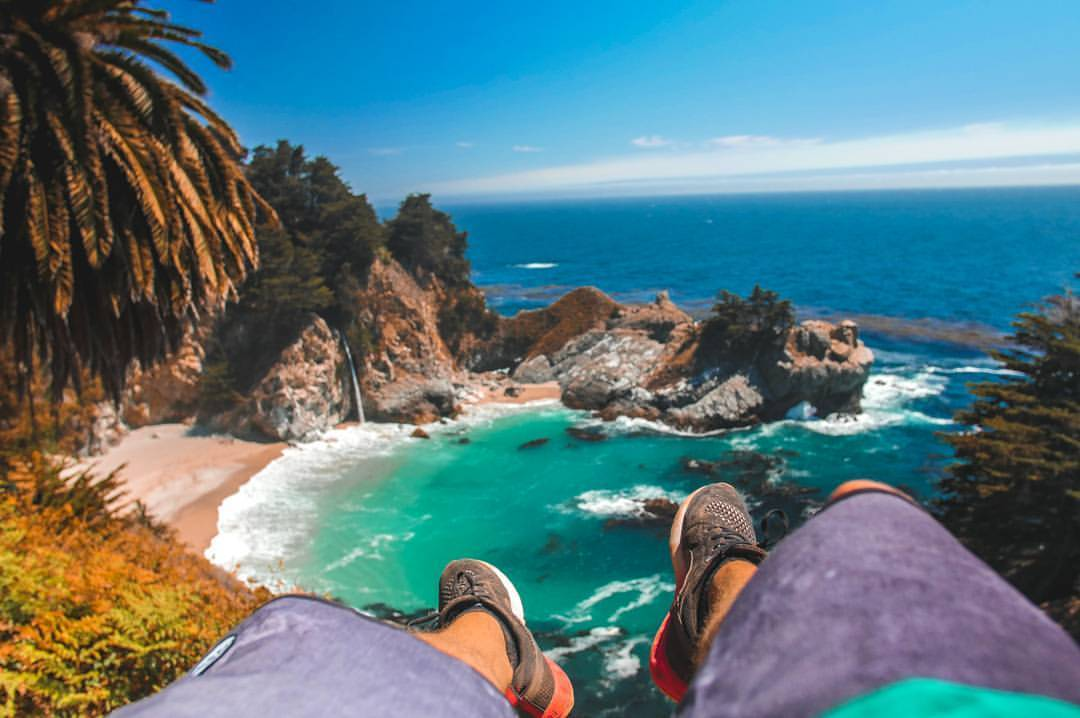
\includegraphics[width=.8\linewidth]{Images/happy.jpg}
  \caption{\textbf{Happy}: ``Just relax with this amazing view \#bigsur \#california \#roadtrip \#usa \#life \#fitness (at McWay Falls)"}
\end{subfigure}
\begin{subfigure}[t]{.5\textwidth}
  \vskip 0pt 
  \centering
  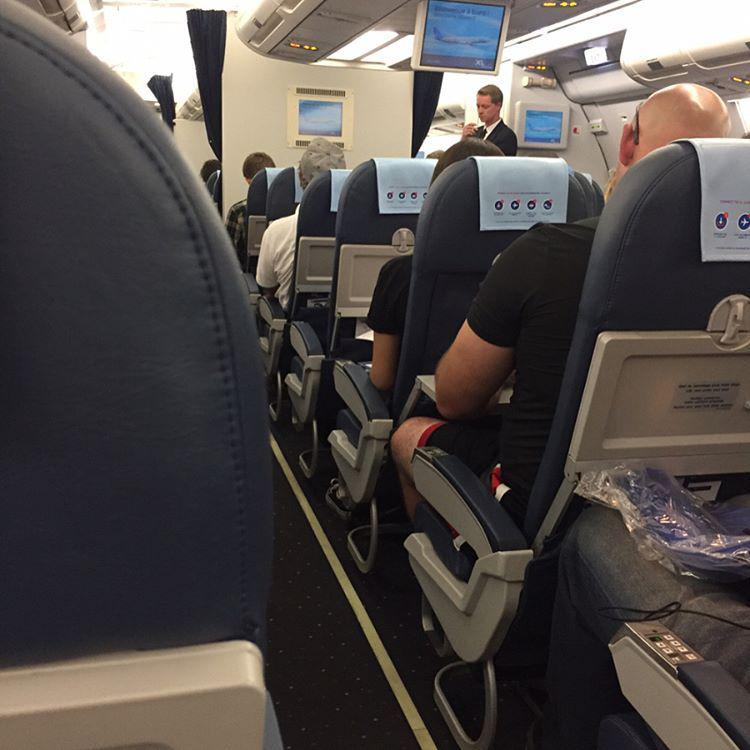
\includegraphics[width=.7\linewidth]{Images/scared.jpg}
  \caption{\textbf{Scared}: ``On a plane guys! We're about to head out into the sky to Paris, France \#Paris \#trip \#kinda \#nervous \#fun \#vacations"}
\end{subfigure}
\begin{subfigure}[t]{.5\textwidth}
  \vskip 0pt
  \centering
  
\includegraphics[width=.6\linewidth]{Images/sad.jpg}
  \caption{\textbf{Sad}: ``It's okay to be upset. It's okay to not always be happy. It's okay to cry. Never hide your emotions in fear of upsetting others or of being a bother   If you think no one will listen. Then I will."}
\end{subfigure}
\begin{subfigure}[t]{.5\textwidth}
  \vskip 0pt 
  \centering
  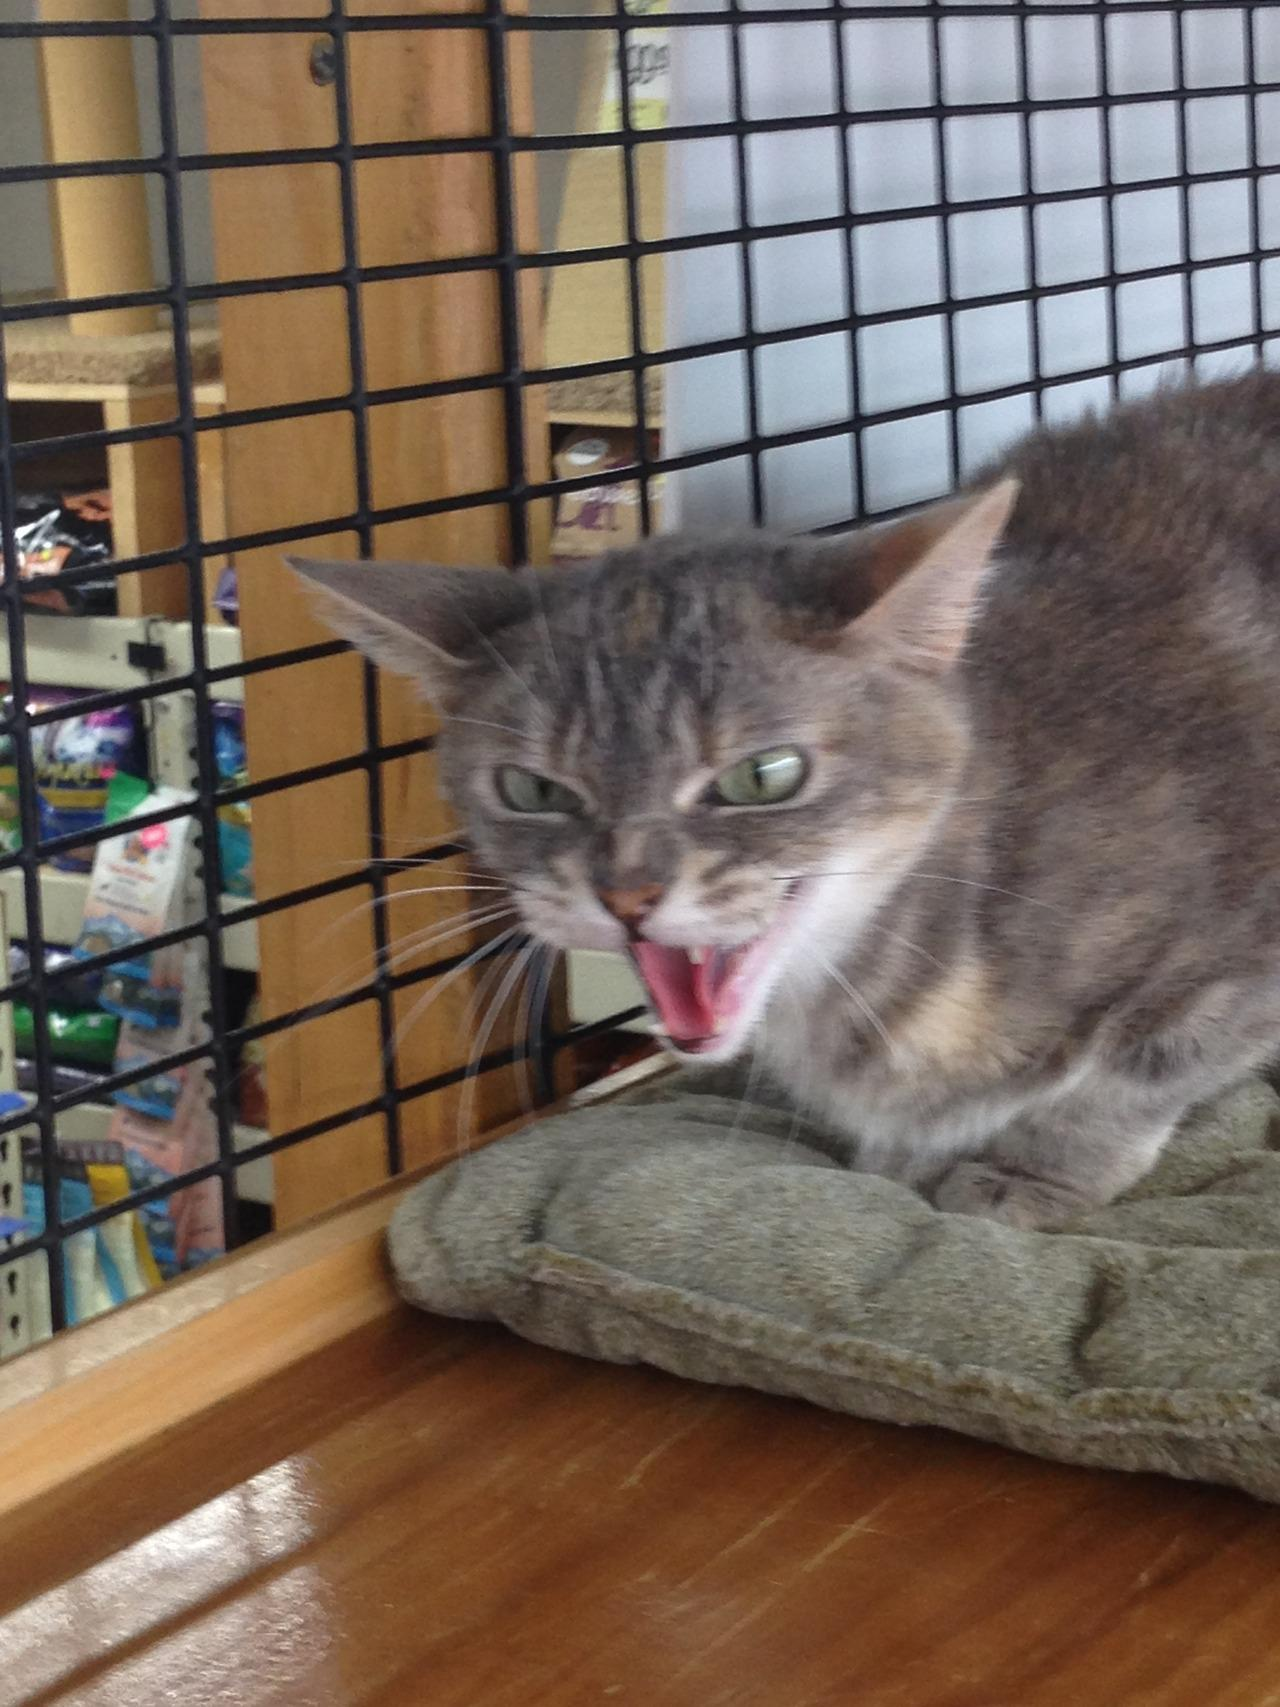
\includegraphics[width=.5\linewidth]{Images/angry.jpg}
  \caption{\textbf{Angry}: ``Tensions were high this Caturday..."}
\end{subfigure}
\begin{subfigure}[t]{.5\textwidth}
  \vskip 0pt 
  \centering
  
\includegraphics[width=.8\linewidth]{Images/surprised.jpg}
  \caption{\textbf{Surprised}: ``Which Tea? Peppermint tea: What is your favorite gif right now?"}
\end{subfigure}
\begin{subfigure}[t]{.5\textwidth}
  \vskip 0pt 
  \centering
  
\includegraphics[width=.8\linewidth]{Images/disgusted.jpg}
  \caption{\textbf{Disgusted}: ``Me when I see a couple expressing their affection in physical ways in public"}
\end{subfigure}
\caption{Some examples of Tumblr posts \cite{tumblr-photos}}
%\label{fig:fig}
\end{figure}